\documentclass[review]{elsarticle}
\usepackage{amsmath}
\usepackage{lineno,hyperref}
\usepackage{siunitx}
\usepackage{csquotes}
\usepackage[table]{xcolor}
\usepackage{slashbox,booktabs}
\usepackage{color}
\usepackage{setspace}
\modulolinenumbers[5]

%\journal{Journal of \LaTeX\ Templates}

%%%%%%%%%%%%%%%%%%%%%%%
%% Elsevier bibliography styles
%%%%%%%%%%%%%%%%%%%%%%%
%% To change the style, put a % in front of the second line of the current style and
%% remove the % from the second line of the style you would like to use.
%%%%%%%%%%%%%%%%%%%%%%%

%% Numbered
%\bibliographystyle{model1-num-names}

%% Numbered without titles
%\bibliographystyle{model1a-num-names}

%% Harvard
%\bibliographystyle{model2-names.bst}\biboptions{authoryear}

%% Vancouver numbered
%\usepackage{numcompress}\bibliographystyle{model3-num-names}

%% Vancouver name/year
%\usepackage{numcompress}\bibliographystyle{model4-names}\biboptions{authoryear}

%% APA style
%\bibliographystyle{model5-names}\biboptions{authoryear}

%% AMA style
%\usepackage{numcompress}\bibliographystyle{model6-num-names}

%% `Elsevier LaTeX' style
\bibliographystyle{elsarticle-num}
%%%%%%%%%%%%%%%%%%%%%%%

\begin{document}

\begin{frontmatter}

\title{A Comparative Study of Texture Analysis Techniques for Osteoarthritis Classification Using Knee X-ray Imagery}
%\tnotetext[mytitlenote]{Fully documented templates are available in the elsarticle package on \href{http://www.ctan.org/tex-archive/macros/latex/contrib/elsarticle}{CTAN}.}

%% Group authors per affiliation:
%\author{Elsevier\fnref{myfootnote}}
%\address{Radarweg 29, Amsterdam}
%\fntext[myfootnote]{Since 1880.}

\author[mymainaddress]{Sophal Chan}
\ead{sophal.c@phuket.psu.ac.th}
\author[mymainaddress]{Kwankamon Dittakan}
\ead{kwankamon.d@phuket.psu.ac.th}
\author[mysecondaryaddress]{Matias Garcia-Constantino}
\ead{m.garcia-constantino@ulster.ac.uk}
%% or include affiliations in footnotes:


%\author[mysecondaryaddress]{Global Customer Service\corref{mycorrespondingauthor}}
\cortext[mycorrespondingauthor]{Corresponding author}
%\ead{support@elsevier.com}

\address[mymainaddress]{College of Computing, Prince of Songkla University, 80, Moo 1, Vichitsongkram Rd, Kathu, Kathu, Phuket, Thailand 83120}
\address[mysecondaryaddress]{School of Computing, Ulster University, Shore Road, Newtownabbey, County Antrim, BT37 0QB, United Kingdom}

\begin{abstract}
Knee Osteoarthritis (OA) is one of the most prominent diseases in aging society and has affected over 10 million people in Thailand. When people suffer from OA it is very difficult to recover back, therefore early detection and prevention are very important. The typical way to detect OA is by using X-ray imaging. This research study is focused on early detection of OA by applying image processing and classification techniques to knee X-ray imagery. The fundamental concept is to find a region of interest, use feature extraction techniques and generate a classifier that is able to distinguish between OA or non-OA images. Firstly, texture analysis is adopted in the research for analyzing the properties of the bone surface of four regions of interest (ROI): (i) Medial Femur (MF), (ii) Lateral Femur (LF), (iii) Medial Tibia (MT), and (iv) Lateral Tibia (LT). Secondly, feature selection is applied to reduce the size of the feature space in terms of number of values and dimensions. Finally, the classifier generator is used to classify imagery between OA and non-OA. The challenge is how to know which regions of interest are suitable to use for the classification process. The data from 131 male and female participants was used for the evaluation while OA imagery was presented as 68 images. The results obtained show that LF is the most appropriate region of interest to consider. Amongst the results obtained for LF, there was an AUC (Area Under the ROC Curve) result of 0.912. The evaluation and results are described in detail.
\end{abstract}

\begin{keyword}
Texture Analysis, Osteoarthritis, Knee OA, Image Classification.
\end{keyword}

\end{frontmatter}

\linenumbers

\section{Introduction}

Osteoarthritis (OA) is a degenerative joint disease which happens in human joints. OA is the most prevalent disease of the joints in the aging society and the most common disease of arthritis which affects millions of people in the United States \cite{Factors2000}. In Thailand the people affected with OA has almost reached 10 million, which is 13\% of Thailand's population, as reported by the National Statistical Office (NSO) in 2014. The NSO also reports that Thailand is going to be an aging society country in ten years. In the aging society, knee OA affects approximately 10\% of men and 13\% of women \cite{BoneandJointInitiativeUSA2014}. Symptoms of knee OA can be detected by the presence of pain, swelling, stiffness in the knee, reduced ability of movement and cracking sound when the knee is moved. Furthermore, OA can be detected early by using medical images to prevent the progression to a more severe stage. Medical imaging that are widely used for OA early detection include: (i) X-ray image, (ii) Computed Tomography (CT) and (iii) Magnetic Resonance Imaging (MRI). The figure below shows knee X-ray images for the (a) Normal and (b) OA cases: \\
\begin{figure}[h]
	\centering
	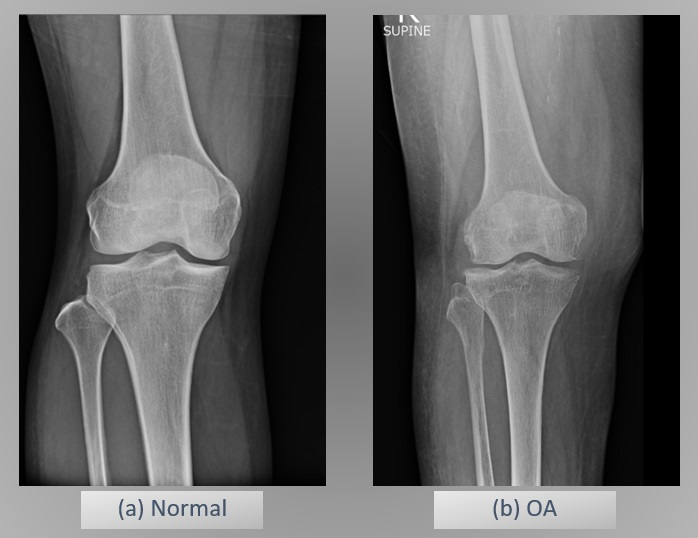
\includegraphics[width=0.7\linewidth]{pic/picOA}
	\caption{Normal and Osteoarthritis (OA) Knee X-ray Imagery.}
	\label{fig:picoa}
\end{figure}



The aim of this research is to apply image processing techniques on medical X-ray images to detect OA. Image processing is a technology in which algorithms can be used to enhance the image or extract some useful features from the image to study for any specific purpose. Image processing is, for example, typically used in fields like: biology, medicine, astronomy and biometrics. In other words, image processing is a specific technology used for: (i) classification, (ii) feature extraction, (iii) multi-scale signal analysis, (iv) pattern recognition and (v) projection. The implementation of image processing for classification in medical X-ray images is proposed in this work. 

The motivation of the research presented is on the classification of the OA and non-OA X-ray images from four sub-images of the knee in terms of the following regions of interest (ROI): (i) Lateral Femur (FM), (ii) Lateral Tibia (LT), (iii) Medial Femur (MF), and (iv) Medial Tibia (MT). The analysis of an image can be done in three main ways including: (i) color-based analysis, (ii) shape analysis, and (iii) texture analysis. Texture analysis is the appropriate way to analyze X-ray images. A texel is the basic unit of a graphic in terms of texture. A texture is a set of texels occurring in some regular or repeated pattern. In other words, texture can produce the information about the spatial arrangement of intensity in an image or selected region of an image. In addition, texture can be analyzed by texture descriptors, which is a technique that can use statistics, filter banks, auto-correlation, etc. The texture descriptors considered in this research work are: (i) histogram feature, (ii) Local Binary Pattern (LBP), (iii) Completed LBP (CLBP), (iv) Rotated LBP (RLBP), (v) LBP Rotation Invariant (LBP\textsubscript{ri}), (vi) LBP Histogram Fourier (LBP-HF), (vii) Local Ternary Pattern (LTP), (viii) Local Configuration Pattern (LCP), (ix) Haralick feature, and (x) Gabor filter feature. As a result, the proposed framework suggested that LBP is the most appropriate texture descriptor for this research study. 

% In addition, the texture feature analysis is used to classify the OA or non-OA in the research while there are 10 techniques of texture analysis are used include: i) The first level of Gray-Level Co-Occurrence Matrix (GLCM), ii) Local Binary Pattern (LBP), iii) Completed LBP (CLBP), iv) Rotated LBP (RLBP), v) LBP Histogram Fourier (LBP\_HF), vi) LBP Rotation Invariant (LBP\_ri), vii) Gabor, viii) Haralick, ix) Local Configuration Pattern (LCP) and x) Local Ternary Pattern (LTP). Next, the ten texture feature descriptor is applied with five different feature selection include: i) Correlation-based Feature Selection (CFS), ii) Chi-square, iii) Gain Ration, iv) Information Gain and v) Relief. Lastly, the learning algorithms are applied to get the final result of the work, learning algorithm is presented in the work include: i) Decision Tree(C 4.5), ii) Decision with binary true, iii) Average One-Dependence Estimators (AODE), iv) Bayesian Network, v) Naïve Bayesian Classifier, vi) Support Vector Machine (SVM), vii) Logistic, viii) Sequential Minimal Optimization, and ix) The backpropagation algorithm.

The proposed technique has three major advantages: (i) fast speed processing, (ii) can be applied in a future study with different imaging modalities, and (iii) can help non-specialist researchers or new profession MDs (Medical Doctors) to analyze OA/non-OA images. On the other hand, the proposed framework still has three main limitations: (i) it is a semi-automatic system which needs an action from a human to chose the ROI, (ii) the dataset is not large enough, and (iii) the result of the experiment is under control from researchers.\\

The remainder of the paper is organised as follows. Section 2 presents related work and Section 3 discusses the proposed framework. Information about each texture feature descriptor is presented in Section 4. Section 5 presents the description of the feature selection and classification algorithms used. Section 6 presents the details about the data collection and Section 7 discusses the evaluation. Finally, conclusions are presented in Section 8. 

\section{Related Work}

In recent years there has been substantial research work in OA detection and classification \cite{Wolski2010, Jin2013, Shamir2009, S.2016, Kotti2017}. The early detection of OA can be applied to medical imaging and used in conjunction with a professional clinician to classify the OA. On the other hand, the implementation of classification techniques to medical imaging for OA detection has been considered as an interesting topic in image processing research fields. Texture is one of the most important properties in images as it shows the arrangement of pixels in objects to analyze. Therefore, texture is one of the useful solutions in medical image processing for diagnosis and detection of OA in a clinical setting \cite{Castellano2004, Janvier2015}. In \cite{Wolski2010}, the research focused on the ROI of tibia texture for the analysis of OA. Texture analysis can be applied to different types of medical images including: X-ray \cite{Wolski2010}, MRI \cite{Chuah2011}, CT, and Infrared \cite{Jin2013}. In addition, the texture of an object can be analyzed using texture descriptors, which is a technique to represent and handle texture in a numeric form. Texture descriptors include: LBP \cite{Castellano2004, Dittakan2016, Kachouie2007}, CLBP \cite{Guo2010}, LBP\textsubscript{ri} \cite{Varney2015}, LBP-HF \cite{Prasad2016}, and LTP \cite{Tan2010, Wang2014}. \\

The study presented in \cite{S.2016} introduced a method to analyze knee OA X-ray images which combined different types of features: (i) shape, (ii) statistical, (iii) Haralick, (iv) texture analysis and (v) first-four moments features. The classification algorithm used in \cite{S.2016} was Random Forest with the data divided into 40\% for training and 60\% for testing. The features considered in \cite{Kawathekar2015} to analyze texture for radiographic OA of knee joint were: (i) entropy, (ii) mean, (iii) median, (iv) standard deviation, (v) variance, and (vi) Tamura texture features. \\

Furthermore, texture analysis has been widely used in the medical field for the detection of various diseases including: tumour heterogeneity \cite{Liu2017, Miles2013}, brain tumour \cite{Weltens2001}, head and neck cancer \cite{Yu2009}, breast cancer \cite{Zhou2007}, emphysema \cite{Xu2006,Vasconcelos}, vascular segmentation \cite{PoddaB.2005, Ahmed2013}, TRUS (transrectal ultrasound) prostate segmentation \cite{Yuan2013, Kachouie2007}, colon cancer \cite{Esgiar2002}, small vessel disease and blood brain barrier \cite{ValdesHernandez2017}, skin cancer \cite{Ntroduction2014}, and lung cancer \cite{Pham2017}.
%LBP is introduced in work [pa], the application of LBP in the work can detected knee OA x-ray image with the implementation of machine learning include: (i) Naïve Bayes, (ii) Decision Tree(C4.5) , (iii) Sequential Minimal Optimisation (SMO), (iv) Back Propagation Neural Networks and (v) Logistic Regression. 

\section{Proposed Framework}

\begin{figure}[h!]
	\centering
	%%\includegraphics[width=0.99\linewidth]{./pic/fig1.png}	
	\includegraphics[width=0.99\linewidth]{./pic/fig1}
	\caption{Texture Analysis on Knee OA Classification Techniques.}
	\label{fig:framework}
\end{figure}

The proposed framework presented in Figure \ref{fig:framework} shows the three main processes considered: (i) Region of interest (ROI) selection, (b) texture extraction, and (c) classification. First and foremost, in order to detect OA/non-OA imagery by using texture analysis it is required to have good quality sub-images of texture. ROI selection is used to select the specific area or sub-image which is considered to have the unique identity for detecting OA by using texture analysis. The ROIs in this process are selected from four different areas as shown in Figure \ref{fig:framework}(a): (i) two on the femur bone on the lateral and medial side, and (ii) two on the tibia on the lateral and medial side. The output of the ROI selection process are the four ROIs: (i) Medial Femur (MF) ROI, (ii) Lateral Femur (LF) ROI, (iii) Medial Tibia (MT) ROI, and (iv) Lateral Tibia (LT) ROI. The output of the ROI selection process is used as the input of the texture extraction process. \\

Texture extraction (refer to Figure \ref{fig:framework}(b)) was used to extract texture of each sub-image from Figure \ref{fig:framework}(a). Feature extraction is a process used to reduce the size of the feature space in terms of the number of values and dimensions. Feature descriptor is a technique widely used to extract features. The research study presented here considered ten different feature extraction techniques, with six of them belonging to the Local Binary Pattern (LBP) family. LBP is a well known texture descriptor technique which is used to analyze the centre pixel in relation to neighboring pixels. In addition to LBP, another six feature descriptors related to LBP applied in this research are: (i) Completed LBP (CLBP), (ii) Rotated LBP (RLBP), (iii) LBP Rotation Invariant (LBP\textsubscript{ri}), (iv) LBP Histogram Fourier (LBP-HF), (v) Local Ternary Pattern (LTP) and (vi) Local Configuration Pattern (LCP). Besides the texture descriptors from the LBP family, the authors implemented three other descriptors: (i) histogram feature, (ii) Haralick feature, and (iii) Gabor filter feature. The implementation of the ten feature descriptors was done in MATLAB. The output of this process is a feature vector which is used as the input of the classification process. \\

Classification is the final process of the proposed framework (refer to Figure \ref{fig:framework}(c)). In order to classify OA/non-OA images, it is required to use machine learning algorithms to process the feature vector generated in the texture extraction process. Nine machine learning algorithms were applied: (i) Decision Tree (C4.5), (ii) Binary Split Tree, (iii) Average One-Dependence Estimators (AODE), (iv) Bayesian Network (BN), (v) Na\"ive Bayes Classifier, (vi) Support Vector Machine (SVM), (vii) Logistic Regression, (viii) Sequential Minimal Optimization (SMO), and (ix) Backpropagation. The implementation of the machine learning algorithms on the feature vector was then evaluated using a number of typically used evaluation measures.

\section{Texture Descriptor}

Texture descriptor is one of the most important techniques to classify the similarity of images. The ten texture feature descriptors used in this research are: \ref{subsec:histogram} histogram feature, \ref{subsec:LBP} Local Binary Pattern (LBP), \ref{subsec:CLBP} Completed LBP (CLBP), \ref{subsec:RLBP} Rotated LBP (RLBP), \ref{subsec:LBPri} LBP Rotation Invariant (LBP\textsubscript{ri}), \ref{subsec:LBP-hf} LBP Histogram Fourier (LBP-HF),  \ref{subsec:LCP} Local Configuration Pattern (LCP), \ref{subsec:LTP} Local Ternary Pattern (LTP), \ref{subsec:haralick} Haralick feature, and \ref{subsec:gabor} Gabor filter feature. The texture descriptors used are described in the following subsections.

\subsection{Histogram feature}
\label{subsec:histogram}
The histogram feature of the grey level image is received by state of the art histogram based feature, it includes:

\begin{itemize}
	\item Mean
	\begin{equation}
	\mu= \sum_{i=1}^N (iP(i))
	\end{equation}
	Where	P(i) is the probability distribution of bin i, which P(i) can be written as: 
	\begin{equation}
	P(i) =\dfrac{H(i)}{M}
	\end{equation}
	\hspace{1cm}H(i) is the histogram function and M is the number of blocks.
	
	
	\item Variance
	\begin{equation}
	\sigma^2= \sum_{i=1}^N (i - \mu)^2P(i)
	\end{equation}
	
	
	\item Skewness \\
	To define the Skewness equation, the standard deviation have to be found first: 
	\begin{equation}
	\sigma = \sqrt{ \sum_{i=1}^N (i - \mu)^2 P(i)}
	\end{equation}
	With the respect to equation (4), the skewness can be defined as: 
	\begin{equation}
	skew = \dfrac{1}{\sigma^3} \sum_{i=1}^N (i - \mu)^3 P(i)
	\end{equation}
	
	\item Kurtosis 
	\begin{equation}
	Kurtosis = \dfrac{1}{\sigma^4} \sum_{i=1}^N (i - \mu)^4 P(i)
	\end{equation}
	
	\item Energy 
	\begin{equation}
	Energy= \sum_{i=1}^N [P(i)]^2
	\end{equation}
	
	
	\item Entropy 
	\begin{equation}
	Entropy= - \sum_{i=1}^N P(i) log_2 [P(i)]
	\end{equation}
\end{itemize}

\subsection{Local Binary Pattern (LBP)}
\label{subsec:LBP}
Local Binary Pattern (LBP) \cite{Ojala1996} is used to label the pixel which is applied thresholding the neighborhood of each pixel with the output as the binary number. The basic functionality of the LBP operator is shown in Figure \ref{fig:LBP} below:

\begin{figure}[h]
	\centering
	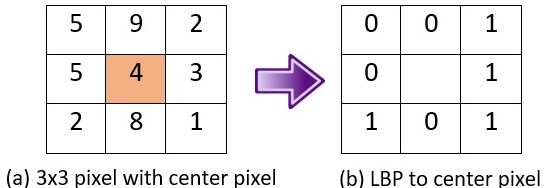
\includegraphics[width=0.6\linewidth]{pic/fig2}
	\caption{LBP Operator.}
	\label{fig:LBP}
\end{figure}
In addition, LBP at pixel (x\textsubscript{c}, y\textsubscript{c}) can be calculated by the equation below:

\begin{equation}
LBP_{P,R} (x_c,y_c) = \sum_{P=0}^{P-1} S(i_P - i_c)2^P
\end{equation}
Where \\ 
P is the pixels surround in the circle neighborhood. \\
R is a radius of circle. \\
i\textsubscript{c}  and i\textsubscript{p}  are the grave-level values of the center point. \\
s(x) is a function which is represented as: \\
\begin{equation}
s(x) = \left\{ \begin{array}{rcl}
1 & \mbox{if}
& x\geq0 \\ 0 & \mbox{if} & x <0 \\

\end{array}\right.
\end{equation}
Besides LBP, there is another LBP texture descriptor called Completed LBP (CLBP) that uses the basic functionality of LBP.

\subsection{Completed LBP (CLBP)}
\label{subsec:CLBP}
In CLBP \cite{Guo2010} a local region is defined by a center pixel and a local difference sign-magnitude transform (LDSMT). This research study is focused on LDSMT, which breaks down the image local structure into two components: (i) the difference signs (CLBP\_S), and (ii) the difference magnitudes (CLBP\_M). The implementation of CLBP\_S and CLBP\_M are shown in Figure \ref{fig:CLBP}: 

\begin{figure}[h!]
	\centering
	\includegraphics[width=0.5\linewidth]{pic/fig3}
	\caption{Example of CLBP Operations.}
	\label{fig:CLBP}
\end{figure}

\subsection{Rotated LBP (RLBP)}
\label{subsec:RLBP}
Rotated LBP (RLBP) \cite{Mehta2013}, sometimes called Dominant Rotated LBP (DRLBP) \cite{Mehta2016} is a rotation technique on LBP around the center pixel. When the reference is in the circular neighborhood token by dominant direction, then the weights are assigned with respect to the dominant direction. Figure \ref{fig:RLBP} shows the implementation of RLBP. 

\begin{figure}[h!]
	\centering
	\includegraphics[width=0.99\linewidth]{pic/fig4}
	\caption{Implementation of RLBP.}
	\label{fig:RLBP}
\end{figure}
The RLBP is defined by the Equation:\\
\begin{equation}
RLBP_{P,R} = \sum_{p=0}^{P-1} S(g_p - g_c)2^{mod(p-D,P)}
\end{equation}

\subsection{LBP Rotation Invariant (LBP\textsubscript{ri})}
\label{subsec:LBPri}
LBP\textsubscript{ri} is the rotation invariant feature which is based on LBP. The LBP operator produces 2P different output values, corresponding to the 2P different binary patterns that can be formed by the P pixels in the neighbor set. In the research study presented we have applied LBP\textsubscript{ri} to each pixel with 8 neighbors, LBP\textsubscript{ri} with 8 bin can be defined by the following equation as:

\begin{equation}
LBP(x,y) = \sum_{P=0}^{7} S(i_P - i_x,y)2^P
\end{equation}

\subsection{LBP Histogram Fourier (LBP-HF)}
\label{subsec:LBP-hf}
LBP-HF is a rotation-invariant image descriptor based on uniform LBPs. The LBP-HF descriptor is formed by first computing a non-invariant LBP histogram over the whole region and then constructing rotationally invariant features from the histogram. LBP-HF is generally used for static features which used Fast Fourier Transform (FFT) to calculate global features from uniform LBP histogram instead of calculating invariant at each pixel independently. This makes the LBP\textsubscript{ri} feature set a subset of LBP-HF. Figure \ref{fig:LBP-HF} shows the implementation of LBP-HF. 

\begin{figure}[h]
	\centering
	\includegraphics[width=0.67\linewidth]{pic/fig5}
	\caption{The implementation of LBP-HF feature for rotation invariant image description.}
	\label{fig:LBP-HF}
\end{figure}

With the respect to Figure 6, 
\texttt{\noindent
	\newline\noindent
	If α=\ang{45}, local binary pattern\\
	\phantom{x}\hspace{10ex}00000010 $\Rightarrow$  00000100 \\
	\phantom{x}\hspace{10ex}00000100 $\Rightarrow$  00001000,...,\\
	\phantom{x}\hspace{10ex}11111000 $\Rightarrow$  11110001,...,\\
	Similarity if α = K * \ang{45}, as a consequence, the pattern have to be circularly rotated with k steps. \\
}




\subsection{Local Configuration Pattern (LCP)}
\label{subsec:LCP}
Local Configuration Pattern (LCP) is a rotation invariant image description technique. LCP decomposes the information architecture of an image into two states: (i) local structural information and (ii) microscopic configuration (MiC). The information consists of image configuration and pixel-wise interaction relationships \cite{Guo2011}. While local structure information is directly related to the basic functionality of LBP, MiC is used for exploring microscopic configuration information. The local structure concept implementation is shown in Figure \ref{fig:LCP}:

\begin{figure}[h!]
	\centering
	\includegraphics[width=0.99\linewidth]{pic/fig6}
	\caption{The concept of LCP.}
	\label{fig:LCP}
\end{figure} 

From Figure \ref{fig:LCP} it can be seen that Figures \ref{fig:LCP}(a) and \ref{fig:LCP}(b) are considered to be of the same pattern type as LBP, but with the implementation of LBP with local invariant information. The patterns shown in Figures \ref{fig:LCP}(a) and \ref{fig:LCP}(b) are different, while the patterns shown in Figures \ref{fig:LCP}(b) and \ref{fig:LCP}(c) are considered to be of the same pattern type due to the same value of variance. In contrast, Figures \ref{fig:LCP}(b) and \ref{fig:LCP}(c) are different in terms of MiC, which MiC based on textural properties. \\

Microscopic configuration information is defined as the modeling of microscopic configuration as expressed in Equation \ref{eq:MCI}: 
\begin{equation}
E(a_0,....,a_{P-1}) = |g_c - \sum_{i=0}^{P-1} a_ig_i|
\label{eq:MCI}
\end{equation}
Where \\
g\textsubscript{c} and g\textsubscript{i} are intensity center pixel values and neighboring pixels.\\
a\textsubscript{i}(i=0,...,P-1) are weighting parameters associated with g\textsubscript{i} \\
E(a\textsubscript{0},...,a\textsubscript{P-1}) is the reconstruction error regarding model parameters of a\textsubscript{i}
\subsection{Local Ternary Pattern (LTP)}
\label{subsec:LTP}
The Local Ternary Pattern (LTP) is based on improving the basic functionality of LBP, which is the analysis of the central pixel i\textsubscript{c} that tends to be sensitive to noise particularly in near-uniform image regions and to smooth weak illumination gradients. LTP can be calculated in gray-level in a zone of width $\pm$ t. The s(x) of LBP is replaced by 3-valued function s\textsubscript{t}(u,i\textsubscript{c},t).

\begin{equation}
s\textsubscript{t}(u,i_c,t) = \left\{ \begin{array}{rcl}
1 & 
& u\geq i_c+t \\ 0 &  & |u - i_c| <t \\
-1 & & u \leq i_c -t

\end{array}\right.
\end{equation}

 \subsection{Haralick feature}
\label{subsec:haralick}

Haralick feature is measured from the Gray-Level Co-occurrence Matrix (GLCM) that is the ordinary way to represent image texture. Haralick feature has been divided into 14 features which are calculated from the statistic of the basic GLCM functionality including: 


\begin{itemize}
	\item Angular Second Moment (ASM)
	\begin{equation}
	ASM = \sum_{i=1}^N\sum_{j=1}^N (P(i,j)^2)
	\end{equation}	
	
	\item Contrast
	\begin{equation}
	Contrast = \sum_{n=0}^{N -1}n^2{\sum_{i=1}^{N}\sum_{j=1}^{N} P(i,j)}, |i - j| =n
	\end{equation}
	
	
	\item Correlation \\ 
	\begin{equation}
	Correlation = \dfrac{\sum_{i=1}^N\sum_{j=1}^N (ij)P(i,j)-\mu_x \mu_y}{\sigma_x \sigma_y} 
	\end{equation}
	
	\item Variance  
	\begin{equation}
	\sigma^2= \sum_{i=1}^N\sum_{j=1}^N (i - \mu)^2P(i,j)
	\end{equation}
	
	\item Inverse Difference Moment (IDM) 
	\begin{equation}
	IDM=\sum_{i=1}^N\sum_{j=1}^N \dfrac{1}{1+(i-j)^2} P(i,j)
	\end{equation}
	
	
	\item Sum Average 
	\begin{equation}
	Sum Average= \sum_{i=2}^{2N} iP_{x+y}(i) 
	\end{equation}
	
	\item Sum Variance
	\begin{equation}
	Sum Variance = \sum_{i=2}^{2N} (i-f_8)^2P_{x+y}(i) 
	\end{equation}
	
	\item Sum Entropy 
	\begin{equation}
	Sum Entropy= - \sum_{i=2}^{2N} P_{x+y}(i) log{P_{x+y}(i)}
	\end{equation}
	
	\item Entropy 
	\begin{equation}
	Entropy= - \sum_{i=1}^N\sum_{j=1}^N P(i,j) log[P(i,j)]
	\end{equation}
	
	\item Difference Variance 
	\begin{equation}
	Difference Variance = \sum_{i=0}^{N-1}i^2 P_{x-y}(i)
	\end{equation}

	\item Difference Entropy 
	\begin{equation}
	Difference Energy= - \sum_{i=0}^{N-1} P{x-y}(i) log [P_{x-y}(i)]
	\end{equation}
	
	\item Information Measure of Correlation 1 (IMC1)
	\begin{equation}
	IMC1= \dfrac{HXY-HXY1}{max{HX,HY}}
	\end{equation}
	
	\item Information Measure of Correlation 2 (IMC2)
	\begin{equation}
	IMC2=\sqrt{ 1-exp[-2(HXY2-HXY)]}
	\end{equation}
	Where 
	\begin{equation}
	\begin{split}
	HXY=- \sum_{i=1}^N \sum_{j=1}^N P(i,j) log(P(i,j)),\\
	HXY1= -\sum_{i=1}^N \sum_{j=1}^N P(i,j) log{P_x(i)P_y(i)},\\
	HXY2=-\sum_{i=1}^N \sum_{j=1}^N P_x(i)P_y(j) log{P_x(i)P_y(j)}
	\end{split}
	\end{equation}
	HX and HY are the entropies of P\textsubscript{x} and P\textsubscript{y}
	
	\item Maximum Correlation Coefficient (MCC) 
	\begin{equation}
	MCC= \sqrt{\sum_{k=1}^N \dfrac{P(i,k)P(j,k)}{P_x(i)P_y(j)}}
	\end{equation}
\end{itemize}


\subsection{Gabor filter feature}
\label{subsec:gabor}
Gabor filter is another texture extraction technique which is used to analyze texture for specific local regions of images with the specific frequency and specific direction. Gabor filter is in fact part of the 2D Gabor filter bank that comprises different parameters including frequencies, orientations and smooth parameters of Gaussian envelope. In addition, Gabor filter bank of pixel (x, y) can be obtained by the Equation \ref{eq:Gabor} below:

\begin{equation}
G(x,y)\equiv e^{-{\dfrac{(x-x_0)^2}{2\sigma^2_x}-\dfrac{(y-y_0)^2}{2\sigma^2_y}}} e^{j(\omega_{x0}x+\omega_{y0}y)}
\label{eq:Gabor}
\end{equation}
where \\
$\omega$\textsubscript{x0}   and   $\omega$\textsubscript{y0} \hspace{0.2cm}   are the centre frequency of x and y direction.\\
$\sigma$\textsubscript{x}    and   $\sigma$\textsubscript{y}   \hspace{0.5cm}  are the standard deviation of the Gaussian function along x and y direction. 

%The author names and affiliations could be formatted in two ways:
%\begin{enumerate}[(1)]
%\item Group the authors per affiliation.
%\item Use footnotes to indicate the affiliations.
%\end{enumerate}
%See the front matter of this document for examples. You are recommended to conform your choice to the journal you are submitting to.

\section{Feature Selection}

Feature selection is one of the most important processes in this research work as it involves the selection of useful features in order to reduce the data dimensionality for the classification process. There are five different feature selection techniques used in this research work: \ref{subsec:CFS} Correlation-based Feature Selection (CFS), \ref{subsec:chi_sq} Chi-Square, \ref{subsec:IG} Information Gain, \ref{subsec:GR} Gain Ratio,  and \ref{subsec:Relief} Relief. Each feature selection technique is described in the following subsections.

\subsection{Correlation-based Feature Selection (CFS)}
\label{subsec:CFS}

Correlation-based Feature Selection (CFS) is a well known feature selection algorithm that uses a heuristic for evaluating the worth of subsets of features. In other words, CFS is used to calculate subsets for the evaluation of features on the basis of the following hypothesis which are based on the heuristic that \textbf{\enquote{Good feature subsets contain features highly correlated with the classification, yet uncorrelated to each other}}  \cite{Hall1999} \cite{Lewandowski2015}. In addition, in CFS it is applied Symmetric Uncertainty, which is the technique used to reduce the redundancy of a feature. The Symmetric Uncertainty which applies to two nominal attributes A and B is given by the equation shown below:
\begin{equation}
U(A,B) =2 \dfrac{H(A)+H(B)-H(A,B)}{H(A) + H(B)}
\label{eq:U_CFS}
\end{equation}
Where \\
H represents the entropy function.\\
H(A, B) the joint entropy of A and B. \\
The value of symmetric uncertainty can start from 0 till 1. 
With respect to Equation \ref{eq:U_CFS}, CFS can be defined as: 
\begin{equation}
	CFS= \dfrac{\sum_{j=i}^m U(A_j,C)}{\sqrt{\sum_{i=1}^m \sum_{j=1}^m U(A_i,A_j)}}
	\label{eq:CFS}
\end{equation}
Where \\
C refers to the class of feature. \\
(A\textsubscript{i}, A\textsubscript{j}) indicates a pair of attributes in the set of features.


\subsection{Chi-Square ($\chi^2$)}
\label{subsec:chi_sq}
In the literature, one way to measure the dependency between a feature and a class is by using Chi-Square ($\chi^2$) feature selection \cite{Plackett1983}. In the implementation of Chi-Square ($\chi^2$), the features are ranked from the most to less useful. Chi-Square ($\chi^2$) is defined by the function shown below:
\begin{equation}
\chi^2 = \sum_{i=1}^{c} \sum_{j=1}^{r} \dfrac{(O_{ij} - E_{ij})^2}{E_{ij}}
\label{eq:chi-sq}
\end{equation}
Where\\
O\textsubscript{ij} is the observed frequency.\\ 
E\textsubscript{ij} is ij is the expected frequency. 


\subsection{Information Gain}
\label{subsec:IG}
Information Gain (IG) measures the amount of information in bits about the class prediction if the only information available is the presence of a feature and the corresponding class distribution \cite{Roobaert}. IG is used to select the test attribute at each node. In other words, IG is a feature evaluation method which is based on entropy \cite{Lei2012}. For example, the IG of a feature t relative to a collection of aspects A, is defined in Equation \ref{eq:IG}: 

\begin{equation}
IG(A,t)=Entropy(A) - \sum_{\substack{v\in Values(t)}} \dfrac{|A_v|}{|A_t|} Entropy(A_v)
\label{eq:IG}
\end{equation}
Where\\
 Values(t) is the set of all possible values for feature t. \\
 A\textsubscript{v} is the subset of S with aspects of class v related to feature t.\\
 A\textsubscript{t} is the set of all aspects belonging to feature t.\\
$\vert$ $\cdot$ $\vert$ refers to the cardinality of a set.

 
\subsection{Gain Ratio}
\label{subsec:GR}
Gain Ratio (GR) is the update or correction of Information Gain (IG). Information Gain is used in a decision tree to select the test attribute at each node \cite{Han2012}. Hence, the implementation of GR to reduce IG bias while choosing an attribute by taking number and size of branches. GR of an attribute (attr) is defined in the equation below: 
 \begin{equation}
 GR(attr)=\dfrac{Gain(attr)}{Entropy(attr)}
 \label{eq:GR}
 \end{equation}
 
\subsection{Relief}
\label{subsec:Relief}

The final feature selection technique considered in this research refers to Relief, which is a weight based algorithm where the relevant features are the ones that have a better distinction between the classes \cite{Kira1994}. Relief works by taking a dataset with n instances of p features which belong to two known classes, each feature of the dataset is scaled to the interval [0 1]. Relief will be repeated m times. Starts with a p-long weight vector (W) of zeros. In other words, Relief computes two weights: namely the near-hit score and the near-miss score based on nearest instances in the neighborhood.
At each repetition of m times, the algorithm takes the feature vector (X) which belongs to one random instance, and the feature vectors of the instance closest to X from each class. The \textbf{\lq Near-hit\rq} is the closest same-class instance, and \textbf{\lq Near-miss\rq} is the closest different-class instance. After m iterations are finished, the algorithm divides each element of the weight vector by m. The relevance vector is created. Features are selected if their relevance is greater than a threshold T.

 
\section{Classification}

Classification is used to identify to which class (OA or non-OA) a new knee X-ray image belongs based on a previously developed classification model. The classification algorithms considered in this research are: \ref{subsec:DT}Decision Tree (C4.5), \ref{subsec:BST} Binary Split Tree, \ref{subsec:AODE} Average One-Dependence Estimators (AODE), \ref{subsec:BN} Bayesian Network (BN), \ref{subsec:Naive} Na\"ive Bayes Classifier, \ref{subsec:SVM} Support Vector Machine (SVM), \ref{subsec:Logistic} Logistic Regression, \ref{subsec:SMO} Sequential Minimal Optimization (SMO), and \ref{subsec:Back} Backpropagation. Each classification algorithm is explained in the following subsections.

\subsection{Decision Tree (C4.5)}
\label{subsec:DT}
Decision tree learning is a well-known classification algorithm used in machine learning \cite{Quinlan1986}. A classification decision tree comprises of the following parts: (i) root node, (ii) internal nodes, and (iii) leaf nodes. The root node is the main root or parent node and has no incoming edges. Internal nodes are used to test on an attribute and the branch defines the output of the test. The leaf nodes, which represent the classes, are the nodes that are at the bottom of the tree and that have no outgoing edges.

\subsection{Binary Split Tree}
\label{subsec:BST}
Binary split tree is the tree in which each node of the tree contains only two values (binary 0-1). The split tree is designed for storing statistic datasets with skewed frequency distributions. The split tree is of the type of decision tree while each node of a decision tree can have multiple values. The split value in the split tree is used for further search in the tree if the key value is not matched to the search value.

\subsection{Average One-Dependence Estimators (AODE)}
\label{subsec:AODE}
Average One-Dependence Estimators (AODE) is a probabilistic classification learning technique which improves the Na\"ive Bayesian classifier \cite{Webb2005} by addressing the problem of attribute-independence. For instance, in the class y, which has a set of features x\textsubscript{1},..., x\textsubscript{n}, AODE can be applied to find the probability of each class y by using the following equation:
	
 	\begin{equation}
 	\hat{P}(y|x_1,...,x_n) = \dfrac{\sum_{i:1\leq i\leq n \wedge F(x_i) \geq m} \hat{P}(y,x_i)\prod_{j=1}^n \hat{P}(x_i|y,x_i)}{ \sum_{y'\in Y}  \sum_{i:1\leq i\leq n \wedge F(x_i) \geq m} \hat{P}(y',x_i) \prod_{i=1}^n \hat{P}(x_j|y',x_i) }
 	\label{AODE}
 	\end{equation}
 	Where \\
 	$\hat{P}$ is an estimate of P \\
 	F  is the frequency \\
 	m is a user specified minimum frequency.

\subsection{Bayesian Network (BN)}
\label{subsec:BN}
Bayesian Network (BN) or Probabilistic Networks (PNs) is a graphical probability model used for reasoning and the decision making in uncertainty \cite{Friedman1998}. In other words, the Bayesian network is a directed acyclic graph (DAG) and each node n $\in$ N of BN represents a domain variable or dataset attribute. In addition, the Bayesian network highly depends on Bayes’ rule. The Bayes' rule can be written as follows: 
 	Assume A\textsubscript{i}  attribute where i= 1,...,n, and take value a\textsubscript{i}  where i= 1,...,n
 	
Assume C as class label attribute and U=(a\textsubscript{1},..., a\textsubscript{n}) as unclassified test instance. U will be classified into class C based on Bayes’ rule is represented as:
 	\begin{equation}
 	P(C|U)=arg\ max P(C)P(U|C)
 	\label{eq:BN}
 	\end{equation}
 	
\subsection{Na\"ive Bayes Classifier}
\label{subsec:Naive}
Na\"ive Bayes is one of the most well-known Bayesian techniques; it uses a simple probabilistic classifier based on the implementation of Bayes' theorem combined with strong (naive) independence assumptions \cite{Lowd2005}. In the related work of Na\"ive Bayes classifier it has been assumed that all the attributes in the same class have been considered as independent given a class label. With respect to Bayes’ rule, the Na\"ive Bayes classifier has been modified as the equation below:
 	\begin{equation}
 	P(C|U) = arg\ max P(C) \prod_{i=1}^n P(A_i|C)
 	\label{eq:Naive}
 	\end{equation}
 	
\subsection{Support Vector Machine (SVM)}
\label{subsec:SVM}
Support Vector Machine (SVM) is a popular linear classifier that has been widely used for the classification task. The objective of SVM is to separate instances of two classes in the most optimal way by constructing an N-dimensional hyperplane between two training sample classes in the feature set \cite{Cortes1995}. SVM classifiers are divided into two categories: (i) linear and (ii) non-linear. They are explained in the following subsubsections. \\

 		\subsubsection{Linear classification}
 		In the case of linear classification, the SVM can be divided into two types of classification: (i) linearly separable case, and (ii) non-linearly separable case. 
 		In the linearly separable case, SVM with the training data {x\textsubscript{i}, y\textsubscript{i}}, y\textsubscript{i} $\in${-1,+1}, i = 1,...,n, can be defined as shown in the equation below: 
		
 		\begin{equation}
 		\left\{ \begin{array}{rcl}
 		x_i . w + b \geq +1 & \mbox{for } 
 		y_i = +1 \\ x_i . w + b \leq -1 & \mbox{for }	y_i = -1
 		
 		\end{array}\right.
 		\label{eq:Linear}
 		\end{equation}
 		In the non-linearly separable case, the SVM equation is changed to: 
 		\begin{equation}
 		\left\{ \begin{array}{rcl}
 		x_i . w + b \geq +1 - \xi_i & \mbox{for } 
 		y_i = +1 \\ x_i . w + b \leq -1 +\xi_i & \mbox{for }	y_i = -1 \\ \xi_i \geq 0, i=1, n
 		
 		\end{array}\right.
 		\label{eq:nonLinear}
 		\end{equation}
 		
 		\subsubsection{Non-linear classification}
		
 		In the case of non-linear classification, the SVM equation can be written as:
		
 		\begin{equation}
 		f(x) = \sum_{i=1}^{n_s} \alpha_i y_i P(x_i,x) +b
 		\label{eq:sum_nonLinear}
 		\end{equation}
 		Where \\
 		n\textsubscript{s} is the number of support vector. \\
 		$\alpha$  is non-negative Lagrange multipliers\\
 		P (x, y) is Polynominal of degree m: k(x,y)=(x.y+1)\textsuperscript{m}
		
\subsection{Logistic Regression}
\label{subsec:Logistic}
Logistic regression is a well-known statistical regression model and it is based on ordinary regression \cite{Wilson2015}. In this research work the logistic regression has been applied to the dependent variable. In addition to this, the logistic regression uses a logistic function, also recognized as the sigmoid function, which is used to compute the logistic model. The logistic model is defined in the following equation:
	
 	\begin{equation}
 	logit(p_t) =x_tb+e_t; p_t=P(y_t =1|x_t,b)
 	\label{eq:logit_PT}
 	\end{equation}
 	Where \\
 	yt ∈ {0,1} 
 	x\textsubscript{t} is the regression vector, x\textsubscript{t} = [1, x\textsubscript{1},x\textsubscript{2},..., x\textsubscript{n}]\\
 	b is the model parameters vector, b = [b\textsubscript{0}, b\textsubscript{1},..., b\textsubscript{n}]’
 	P( | )  is the conditional probability function (pf) and 
 	logit() is the logistic function. The logit() can be represented as: 
 	\begin{equation}
 	logit(p)=ln(\dfrac{p}{1-p})
 	\label{eq:logit_P}
 	\end{equation}
	
\subsection{Sequential Minimal Optimization (SMO)}
\label{subsec:SMO}
Sequential Minimal Optimization (SMO) is the improvement from SVM to solve the quadratic programming (QP) optimization problem, which happens during the SVM training \cite{Platt1998}. Furthermore, the QP optimization problem can be represented while SVM finds $\alpha_i$, as the equation below:

 	\begin{equation}
 	min \ L_D(\alpha)= \sum_{i=1}^n \alpha_i -\dfrac{1}{2}\sum_{i=1}^n \sum_{j=1}^n \alpha_i \alpha_j y_iy_j(x_ix_j)
 	\label{eq:minLD}
 	\end{equation}
 	
 	\begin{equation}
 	s.t \ 0 \leq \alpha_i \leq C \quad  and \quad \sum_i^n \alpha_i y_i =0, \quad \forall i
    \label{eq:st}
 	\end{equation}
 	With respect to the two equations above \ref{eq:minLD} and \ref{eq:st}, SMO selects and solves the Smallest Optimization Problem (SOP).
	
\subsection{Backpropagation}
\label{subsec:Back}
The backpropagation algorithm is widely known and used in neural networks to calculate a gradient which is required in the calculation of the weights to be used in the network \cite{Kelley1960}. In other words, backpropagation is learning the same as the neural network, which is finding the minimum of the error function.

\section{Data Collection}

In this section, the knee X-ray dataset collection and the analysis of region of interest (RoI) of knee for classification are presented.

\subsection{Dataset}

The dataset used in this research work was collected from 2 local hospitals in Thailand. The number of images used was 131 and they were divided as follows: (i) 63 non-OA images, and (ii) 68 OA images. To protect the data privacy of the patients that participated in this study, for each image collected only the image data was used, thus excluding personal information (e.g. age, gender, address, etc.).

\subsection{Region of Interest (ROI)}

Four different places in the knee X-ray images were identified and used as ROI for texture analysis, they are shown in Figure 8: \\

\begin{figure}[h]
	\centering
	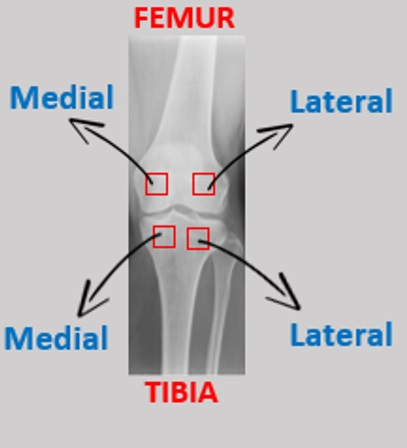
\includegraphics[width=0.5\linewidth]{pic/fig9}
	\caption{The Four ROI of Texture Analysis}
	\label{fig:fig9}
\end{figure}

In relation to the four ROIs identified from the X-ray images, the collected dataset was divided into four datasets, each one containing the 131 images focused on the respective ROI: (i) Medial Femur (MF) dataset, (ii) Lateral Femur (LF) dataset, (iii) Medial Tibia (MT) dataset, and (iv) Lateral Tibia (LT) dataset. The four ROI datasets were used for analysis and evaluation using image processing and classification techniques.

\section{Evaluation}

The evaluation of the proposed approach to OA screening is presented in this section. While 7,272 experiments were conducted with respect to the proposed approach, only the most significant results obtained are presented. The evaluation was conducted by considering a case study directed at 131 digital X-ray images taken in Postero-Anterior (PA) position. The dataset comprised: (i) X control (normal) and (ii) Y OA images. Ten-Fold Cross-Validation (TCV) was applied throughout. The evaluation measures used were: (i) Area Under the ROC Curve (AUC), (ii) Accuracy (AC), (iii) Sensitivity (SN), (iv) Specificity (SP), (v) Precision (PR), and (vi) F-Measure (FM). The overall aim of the evaluation was to provide evidence that the OA condition can be easily detected using the proposed framework. To this end four sets of experiments were conducted with the objectives of comparing and selecting the best results for the following criteria:

\begin{enumerate}
\item Region of Interest (ROI)
\item Texture descriptor
\item Feature selection technique
\item Classification algorithm
\end{enumerate}

%\singlespacing1. Identify the best ROI from the best experiment result. 
%\singlespacing2. Compare of the best feature descriptor for the research experiment. 
%\singlespacing3. Studying the best feature selection technique for experiment.
%\singlespacing4. Selection learning algorithm for the best classification result. \\ \\

%For each objective is presented detail in sub-section 8.1-8.4:

The comparison and results for each area of interest is presented in the following subsections.

\subsection{Region of Interest (ROI) results}

The classification results presented in this subsection are with respect to the four ROIs considered and used for texture analysis: (i) Medial Femur (MF), (ii) Lateral Femur (LF), (iii) Medial Tibia (MT), and (iv) Lateral Tibia (LT). Note that for each ROI a dataset of 131 digital X-ray images focused on the respective ROI was used. The results obtained are presented in Table \ref{tab:ROIResult}. \\

%\begin {tabular}{|l|>{$}c<{$}|>{$}c<{$}|}\hline
%\backslashbox{ROI}{Algorithm} &AUC&AC&SN&SP&PR&FM\\\hline
%Literal Femur(LF) & 0 & 1\\\hline
%Medial Femur(MF) & 1 & 0\\\hline
%\end{tabular}
\begin{table}[h]
	\centering
\begin{tabular}{|c|c|c|c|c|c|c|}
	\hline 
\backslashbox{ROI}{Algorithm} &AUC&AC&SN&SP&PR&FM\\
	\hline
	Medial Femur (MF)	& 0.884 & 0.794 & 0.794 & 0.792  & 0.794  & 0.794  \\ 
	\hline 
\cellcolor{blue!25}Lateral Femur (LF)	&\cellcolor{blue!25} 0.912 &\cellcolor{blue!25} 0.832  & \cellcolor{blue!25}0.832 &\cellcolor{blue!25}0.832  &\cellcolor{blue!25}0.832  & \cellcolor{blue!25}0.832 \\
	\hline 
Medial Tibia (MT)	& 0.895  & 0.802  & 0.802  & 0.802  & 0.802  & 0.802  \\
	\hline 
Lateral Tibia (LT)	& 0.883  & 0.809  & 0.809 & 0.809  & 0.809  & 0.809  \\
	\hline 
\end{tabular} 
\caption{Region of Interest (ROI) results.}
\label{tab:ROIResult}
\end{table}

The best classification results for the ROIs was obtained when the Local Binary Pattern (LBP) feature descriptor was applied combined with the Bayesian Network classification algorithm. In terms of ROI, although the results of all the ROIs can be considered as good, the best classification result was obtained by the Lateral Femur (LF) ROI with an AUC value of 0.912.

\subsection{Texture descriptor results}

The classification results presented in this subsection are with respect to the Lateral Femur (LF) ROI, which obtained the best results amongst the ROIs, and the texture descriptors. The ten texture descriptors considered were: (i) histogram feature, (ii) Local Binary Pattern (LBP), (iii) Completed LBP (CLBP), (iv) Rotated LBP (RLBP), (v) LBP rotation invariant (LBP\textsubscript{ri}), (vi) LBP histogram Fourier (LBP-HF), (vii) Local Ternary Pattern (LTP), (viii) Local Configuration Pattern (LCP), (ix) Haralick feature, and (x) Gabor filter feature. The results obtained are shown in Table \ref{tab:TextureResult}. \\

\begin{table}[h!]
	\centering
	\begin{tabular}{|c|c|c|c|c|c|c|}
		\hline 
		\backslashbox{Texture \\ Descriptor}{Algorithm} &AUC&AC&SN&SP&PR&FM\\
		\hline 
		Histogram	& 0.757 & 0.695  & 0.695 & 0.69  & 0.695  & 0.693 \\ 
		\hline
		\cellcolor{blue!25}	LBP 		&\cellcolor{blue!25}0.912  &\cellcolor{blue!25}0.832  &\cellcolor{blue!25}0.832  &\cellcolor{blue!25}0.832  &\cellcolor{blue!25}0.832  &\cellcolor{blue!25}0.832  \\
		\hline
		CLBP		& 0.882 & 0.763 & 0.763 & 0.762  & 0.763  & 0.763  \\ 
		\hline
		RLBP	 	& 0.895  & 0.809  & 0.809  & 0.81  & 0.81  & 0.809  \\
		\hline
		LBP\textsubscript{ri}	& 0.812  & 0.771  & 0.771  & 0.771  & 0.771  & 0.771  \\
		\hline
		LBP-HF 		& 0.773  & 0.71  & 0.71  & 0.717  & 0.71  & 0.709  \\ 
		\hline
		LTP		 	& 0.816  & 0.756  & 0.756  & 0.761  & 0.763  & 0.755  \\
		\hline
		LCP		 	& 0.783  & 0.725  & 0.725  & 0.724  & 0.725  & 0.725  \\
		\hline
		Haralick 	& 0.695  & 0.664  & 0.664  & 0.67  & 0.672  & 0.662  \\
		\hline
		Gabor		& 0.883  & 0.786  & 0.786  & 0.786  & 0.786  & 0.786  \\ 
		\hline
	\end{tabular} 
	\caption{Texture descriptor results.}
	\label{tab:TextureResult}
\end{table}

Although most of the results obtained with different texture descriptors can be considered as good, the results that stand out are the ones obtained using the LBP texture descriptor. The worst results, on the other hand, were obtained by the Haralick feature with an AUC of 0.695.

\subsection{Feature selection technique results}

In this subsection the classification results are presented in terms of the following feature selection techniques: (i) Correlation-based Feature Selection (CFS), (ii) Chi-Square, (iii) Gain Ratio, (iv) Information Gain, and (v) Relief. The results obtained are presented in Table \ref{tab:FeatureResult}.

\begin{table}[h!]
	\centering
	\begin{tabular}{|c|c|c|c|c|c|c|}
		\hline 
		\backslashbox{Texture \\ Selector}{Algorithm} &AUC&AC&SN&SP&PR&FM\\
		\hline 
	\cellcolor{blue!25}CFS			& \cellcolor{blue!25} 0.912 & \cellcolor{blue!25}0.832  & \cellcolor{blue!25}0.832 & \cellcolor{blue!25}0.832  & \cellcolor{blue!25}0.832  & \cellcolor{blue!25}0.832 \\ 
		\hline 
		Chi-Square	& 0.699 & 0.687 & 0.687 & 0.687  & 0.687  & 0.687  \\ 
		\hline 
		Gain Ratio		& 0.709  & 0.687  & 0.687  & 0.687  & 0.687  & 0.687  \\ 
		\hline 
		Information Gain 	& 0.699  & 0.687  & 0.687  & 0.684  & 0.687  & 0.687 \\ 
		\hline 
		Relief 		& 0.699  & 0.679  & 0.679  & 0.674 & 0.681  & 0.677  \\ 
		\hline
	\end{tabular} 
	\caption{Feature selection technique results.}
	\label{tab:FeatureResult}
\end{table}

The best AUC classification results in terms of feature selection technique were obtained by CFS for the LF RoI in the case of using the LBP texture descriptor and the Bayesian Network classification algorithm. The second best classification results were obtained by the Gain Ratio feature selection technique for the LT RoI with an AUC of 0.709, using the LBP\textsubscript{ri} and the Decision Tree binary tree classification algorithm. The AUC results obtained for the Chi-Square, Information Gain and Relief feature selection techniques were the same. The results obtained for the Chi-square, Information Gain, and Relief feature selection technique were obtained by using histogram feature and the Na\"ive Bayes Classifier from LF RoI. 

%With reference to table 3, the best result of CFS in the highlight color can be founded out by LF applied with LBP and Bayes Network, while Chi-square result is presented by LF applied with GLCM and Naïve Bayes for AUC value and others value from MT applied with CLBP and decision tree. For the gain ratio, the best result, have founded by LT applied with LBP\_ri and decision tree binary true, and others value are pointed out by LT applied with LTP and SMO. In the information gain, the best result is presented by LF applied with histogram feature and Naïve Bayes, while others value by LT applied with LTP and SMO. Lastly, the best result of Relief is received from LF applied with histogram feature and Naïve Bayes. The best result of the learning algorithm is presented in next subsection.

\subsection{Classification algorithm results}

In this subsection the classification results are presented considering the classification algorithms used. The results obtained are presented in Table 4.

\begin{table}[h!]
	\centering
	\begin{tabular}{|c|c|c|c|c|c|c|}
		\hline 
		\backslashbox{Machine Learning \\ Algorithm}{Algorithm} &AUC&AC&SN&SP&PR&FM\\
		\hline  
		C4.5		& 0.757 &	0.779 &	0.779 &	0.78 &	0.78 &	0.779\\
		\hline
		Binary Split Tree	& 0.766	& 0.74	& 0.74	& 0.736	& 0.742	& 0.739 \\
		\hline 
		AODE	& 0.896	& 0.809	& 0.809	& 0.804	& 0.809	& 0.809 \\
		\hline 
	\cellcolor{blue!25}	Bayesian Network	& \cellcolor{blue!25}0.912	& \cellcolor{blue!25}0.832	& \cellcolor{blue!25}0.832	& \cellcolor{blue!25}0.832	& \cellcolor{blue!25}0.832	& \cellcolor{blue!25}0.832\\
		\hline 
		Na\"ive Bayes	& 0.903	& 0.817	& 0.817	& 0.816	& 0.817	& 0.817 \\
		\hline 
		SVM			& 0.715	& 0.718	& 0.718	& 0.711	& 0.72	& 0.715 \\
		\hline 
		Logistic Regression	& 0.904	& 0.84	& 0.84	& 0.844	& 0.847	& 0.839 \\
		\hline 
		SMO			& 0.771	& 0.771	& 0.771	& 0.771	& 0.771	& 0.771 \\
		\hline 
		Backpropagation	& 0.851	& 0.771	& 0.771	& 0.77	& 0.771	& 0.771 \\
		\hline 
	\end{tabular} 
	\caption{Classification algorithm results.}
	\label{tab:AlgorithmResult}
\end{table}

From Table \ref{tab:AlgorithmResult}, the best results of learning classification algorithms are presented. The top three AUC classification results of learning algorithms include: (i) the best one was the Bayesian Network algorithm with the value of 0.912, (ii)the second best was the Logistic Regression and (iii) the third best was the Na\"ive Bayes Classifier. Regarding the best AC result: (i) Logistic Regression obtained 0.84, (ii) the second best result was obtained with Bayesian Network, and (iii) the third best was the Na\"ive Bayes Classifier. Hence, the three most efficient learning algorithms were: (i) Bayesian Network, (ii) Logistic Regression and (iii) Na\"ive Bayes Classifier. Based on the AUC results obtained with Bayesian Network, Logistic Regression and Na\"ive Bayes, the best results of the research were obtained by LF RoI applied with LBP and CFS. Table \ref{tab:AlgorithmResult} also shows the results obtained by the other six classification algorithms ordered from high to low with respect to their AUC results: (i) AODE, (ii) Backpropagation, (iii) SMO, (iv) Binary Split Tree, (v) Decision tree, and (vi) SVM. 




 %the best result of decision tree have gained by the implementation of MT applied with CLBP and CFS, while decision tree with the binary true best result is pointed out by LT applied with LBP and CFS for AUC value and others from LTP applied with LTP and CFS. For the AODE result is presented by LF applied with LBP and CFS for AUC value, LT applied with LBP and CFS for SP value, and others are founded by LT or LF applied with LBP and CFS. The implementation of LF applied with LBP and CFS have produced the best result of Bayes Network, while the best result of Naïve bay is produced by LF applied with LBP and CFS for AUC value and others values by LT applied with LBP and CFS. Furthermore, the best result of SVM can be founded out by the implementation of LF applied with LBP\_ri and CFS, while the logistic result is presented by the implementation of LF applied with LBP and CFS. For the SMO best result is a reference to the implementation of LF applied with RLBP and CFS. Lastly, the multilayer finds out by LF applied with RLBP and CFS for AUC, LT and others are applied from LF applied with LBP\_ri with CFS.

\section{Conclusions}

Early detection of OA by applying image processing and classification techniques to human knee X-ray imagery was presented. The detection was applied with the difference of four sub-images: (i) Lateral Femur (LF), (ii) Lateral Tibia (LT), (iii) Medial Femur (MF), and (iv) Medial Tibia (MT). In addition, in order to carry out a more comprehensive research study, ten type of texture descriptors were applied to the sub-imagery of X-ray images, for example: (i) Histogram feature, (ii) Local Binary Pattern (LBP), (iii) Completed LBP (CLBP), (iv) Rotated LBP (RLBP), (v) LBP Histogram Fourier (LBP-HF), (vi) LBP Rotation Invariant (LBP\textsubscript{ri}), (vii) Gabor, (viii) Haralick, (ix) Local Configuration Pattern (LCP), and (x) Local Ternary Pattern (LTP). The implementation of feature selection was presented to reduce the dimension and space of the features from each feature descriptor. For the feature selection technique, the research study applied five well-known techniques: (i) Correlation-based Feature Selection (CFS), (ii) Chi-square, (iii) Gain
Ratio, (iv) Information Gain, and (v) Relief. The last part of the study focused on the implementation of nine machine learning classification algorithms: (i) Decision Tree (C4.5), (ii) Decision with binary tree, (iii) Average One-Dependence Estimators (AODE), (iv) Bayesian Network, (v) Na\"ive Bayesian Classifier, (vi) Support Vector Machine (SVM), (vii) Logistic Regression, (viii) Sequential Minimal Optimization (SMO), and (ix) the Backpropagation algorithm. The classification results of the research were evaluated by six different evaluation measures: (i) Area Under the ROC Curve (AUC), (ii) Accuracy (AC), (iii) Sensitivity (SN), (iv) Specificity (SP), (v) Precision (PR), and (vi) F-Measure (FM).

The best classification result obtained had an AUC value at 0.912. With the best result of the research study presented, four main interesting aspects can be identified:

\begin{itemize}
\item Regarding the amount of four sub-imagery of knee image, the Lateral Femur (LF) produce a better performance of classification in terms of the implementation of LBP with Bayesian Network.
\item In the implementation of the ten texture descriptors, only LBP produced the AUC value at 0.912, which was the highest value recorded in the study.
\item The best performance of feature selection for classification was recorded by CFS with five well-known feature selection techniques.
\item The most efficient learning algorithm for classification was performed by Bayesian Network.
\item The highest AUC value of 0.912 was recorded by the implementation of 4 parameters: (i) Lateral Femur sub-image, (ii) LBP descriptor, (iii) CFS feature selector, and (iv) Bayesian Network algorithm.
\end{itemize}

Future work considered includes using a larger dataset and implementing Convolutional Neural Network (CNN), which is a small branch of Deep Learning that can remove the feature selection process for learning OA/Normal classification imagery.

\section{Acknowledgement}

We would like to express our gratitude to the Bangkok hospital Phuket branch and Dibuk hospital for providing the X-ray dataset used in this research study. We would like to give special thanks to MD. Sirisak Yaisoongnern for managing the process of data collection and million thanks to MD. Chaowakon Saehang for sharing his valuable knowledge in OA grading field.

\section*{References}

\bibliography{normalOA}

\end{document}